\documentclass{thesisclass}

%% -------------------------------
%% |  Information for PDF file   |
%% -------------------------------
\hypersetup{
    colorlinks=false,
    linkbordercolor={0.6353 0.1333 0.1373}, %KIT red
    filebordercolor={0.1373 0.6314 0.8784}, % KIT cyan 
    urlbordercolor={0.2745 0.3922 0.6667}, % KIT blue
    citebordercolor={0 0.5882 0.5098}, % KIT green
    pdftitle={Improvement of the single top-quark detection in the s-channel at the CMS Experiment},
    pdfauthor={Genti Saliu},
    pdfkeywords={none}
}

%% ---------------------------------
%% | Information about the thesis  |
%% ---------------------------------
\newcommand{\myname}{Genti Saliu}
\newcommand{\mytitle}{Improvement of the single top-quark detection in the s-channel at the CMS Experiment}
\newcommand{\myinstitute}{Institute of Experimental Particle Physics}
\newcommand{\mydepartment}{Department of Physics}
\newcommand{\myuniversity}{Karlsruhe Institute of Technology (KIT)}
\newcommand{\myplace}{Karlsruhe}

\newcommand{\reviewerone}{Prof. Dr. Thomas Müller}
\newcommand{\reviewertwo}{Dr. Nils Faltermann}
\newcommand{\timestart}{08 August 2018}
\newcommand{\timeend}{08 November 2018}
\newcommand{\submissiontime}{08 November 2018}

%%%%%%%%%%%%%%%%%%%%%%%%%%%%%%%%%
%% Here, main documents begins %%
%%%%%%%%%%%%%%%%%%%%%%%%%%%%%%%%%
\begin{document}

\selectlanguage{english}

\frontmatter
\pagenumbering{roman}
%% titlepage.tex
%%

% coordinates for the bg shape on the titlepage
\newcommand{\diameter}{20}
\newcommand{\xone}{-15}
\newcommand{\xtwo}{160}
\newcommand{\yone}{15}
\newcommand{\ytwo}{-253}

\begin{titlepage}
% bg shape
\begin{tikzpicture}[overlay]
\draw[color=gray]  
 		 (\xone mm, \yone mm)
  -- (\xtwo mm, \yone mm)
 arc (90:0:\diameter pt) 
  -- (\xtwo mm + \diameter pt , \ytwo mm) 
	-- (\xone mm + \diameter pt , \ytwo mm)
 arc (270:180:\diameter pt)
	-- (\xone mm, \yone mm);
\end{tikzpicture}
	\begin{textblock}{10}[0,0](4,2.5)
		
\includegraphics[width=.3\textwidth]{assets/LogoKit.pdf}
	\end{textblock}
        \begin{textblock}{11.9}[0,0](3.5,2.5)
          \changefont{phv}{m}{n}
          \raggedleft{\Large{ETP\_Bachelor\_2018\_21}}
        \end{textblock}
	\changefont{phv}{m}{n}	% helvetica	
	\vspace*{3.5cm}
	\begin{center}
		\Huge{\mytitle}
		\vspace*{1cm}\\
		\vspace*{2cm}
		\Large{Bachelor Thesis}\\
		\vspace*{1cm}
		\huge{\myname}\\
		\vspace*{1cm}
		\Large{At the \mydepartment
			\\
			\myinstitute
		}
	\end{center}
	\vspace*{1cm}
\Large{
\begin{center}
\begin{tabular}[ht]{l c l}
  % Gutachter sind die Professoren, die die Arbeit bewerten. 
  \iflanguage{english}{Reviewer}{Erstgutachter}: & \hfill  & \reviewerone\\
  \iflanguage{english}{Second reviewer}{Zweitgutachter}: & \hfill  & \reviewertwo%\\
  %\iflanguage{english}{Advisor}{Betreuender Mitarbeiter}: & \hfill  & \advisor\\
  %\iflanguage{english}{Second advisor}{Zweiter betreuender Mitarbeiter}: & \hfill  & \advisortwo\\
  % Der zweite betreuende Mitarbeiter kann weggelassen werden. 
\end{tabular}
\end{center}
}


\vspace{2cm}
\begin{center}
%\large{\iflanguage{english}{Duration:}{Bearbeitungszeit}: \timestart
%\hspace*{0.25cm} -- \hspace*{0.25cm} \timeend}
\large{\myplace, \timeend}
\end{center}


\begin{textblock}{10}[0,0](4,16.8)
\tiny{ 
	\iflanguage{english}
		{KIT -- University of the State of Baden-Wuerttemberg and National Research Center of the Helmholtz Association}
		{KIT -- Universit\"at des Landes Baden-W\"urttemberg und nationales Forschungszentrum in der Helmholtz-Gemeinschaft}
}
\end{textblock}

\begin{textblock}{10}[0,0](14,16.75)
\large{
	\textbf{www.kit.edu} 
}
\end{textblock}

\end{titlepage}

\vspace*{\fill}

\rule{1.0\textwidth}{0.6pt}

\vspace*{0.75em}

Accepted by the first reviewer of the bachelor thesis.

\textbf{\myplace, \submissiontime}

\vspace*{4em}

\dotfill \hspace*{8cm} 

\hspace*{0.82cm}(\textbf{\reviewerone})

\vspace*{\fill}

\rule{1.0\textwidth}{0.6pt}

\vspace*{0.75em}

I hereby certify that the enclosed thesis is my own work, that I have not sought or used inadmissible help of third parties to produce this work and that I have clearly referenced all sources used in the text.

\vspace*{0.75em}

\textbf{\myplace, \submissiontime}

\vspace*{4em}

\dotfill \hspace*{8cm} 

\hspace*{1.79cm}(\textbf{\myname})

\blankpage


%% -------------------
%% |   Directories   |
%% -------------------
\tableofcontents
\blankpage


%% -----------------
%% |   Main part   |
%% -----------------
\mainmatter
\pagenumbering{arabic}
\chapter*{Abstract}

The top quark was the last quark in the standard model of particle physics to be discovered in 1995. It is with a mass of \SI{173}{GeV} the heaviest elementary particle in the standard model and the only quark with a mass on the same order as the electroweak symmetry breaking scale. The large mass was the cause for its late discovery, as particle accelerators with high center-of-mass energies are needed.

At the Large Hadron Collider, top quarks are predominantly produced in pairs through the strong interaction with a smaller portion being produced individually via the electroweak interaction through the $s$ channel, the $t$ channel or in the associated production with a \PW boson.

The study of $s$-channel single top quark production is important in exploring the electroweak sector of the standard model. Deviations from the standard model prediction of its cross section may hint to physics beyond the standard model (BSM) \cite{CMS16}. $s$-channel single top quark production accounts only for a small proportion of the total production of top quarks. Therefore, a good separation between signal and background events is required, with single top quarks produced via the $s$-channel constituting signal and top quark pairs (\PtopNOSPACE\APtop) background events. 

This thesis explores the improvement of the reconstruction of $s$-channel produced single top quarks over methods used so far by employing a feed-forward neural network classifier. Monte Carlo simulations for the Compact Muon Solenoid Experiment from 2017 are used to train and test the neural network. Several machine learning techniques are employed in choosing suitable input variables for the neural network and optimizing the topology of the neural network. The classifier presented in this thesis achieves an over \SI{7}{\%} improvement upon the existing reconstruction methods. It is expected that with an improved reconstruction a better separation between signal and background events can be realized.
\chapter{Theoretical Background}
\label{ch:theory}

This chapter discusses the theory relevant for the thesis. Section \ref{sec:theory_sm} provides an overview of the standard model (SM) of particle physics, the context for this work. Section \ref{sec:theory_top} focuses on properties of the top quark, its production processes and decay modes, which are important in the development and evaluation of the classifier in chapter \ref{ch:classifier}. Throughout this thesis natural units ($\hbar=c=1$) are used.

\section{The Standard Model of Particle Physics}
\label{sec:theory_sm}
The SM describes the known elementary particles and their interactions. Elementary particles are categorized in fermions and bosons based on their spin quantum number.

\textbf{Fermions} are particles with a spin of $\nicefrac{1}{2}$. They are grouped into six quarks and six leptons, which are arranged according to their masses in three generations. The quarks are named the up (\Pup), down (\Pdown), charm (\Pcharm), strange (\Pstrange), top (\Ptop) and bottom (\Pbottom) quark. The leptons are the electron (\Pe), electron neutrino (\Pelectronneutrino), muon (\Pmuon), muon neutrino (\Pmuonneutrino), tau (\Ptau), and tau neutrino (\Ptauneutrino). For each fermion an antifermion with equal mass, but opposite electric charge, color, and third component of isospin, exists. A summary of the fermions is given in Table \ref{tab:ch_1_sm_fermions}.

\begin{table}[h]
    \caption[Fermions of the Standard Model]{Six leptons and six quarks constitute the fermions of the SM. The particles are ordered according to their generation. Source: \cite{Pov14}}
    \label{tab:ch_1_sm_fermions}
    \begin{center}
        \begin{tabular}{ccccccccc}
            \toprule
            \multirow{2}{*}{Fermions} & \multicolumn{3}{c}{Generation} & {Electric} & \multirow{2}{*}{Color} & \multirow{2}{*}{Isospin $I_3$} & \multirow{2}{*}{Spin}\\
            & 1 & 2 & 3 & {charge} & & & \\
            \midrule
            \multirow{2}{*}{Leptons} & \Pelectronneutrino & \Pmuonneutrino & \Ptauneutrino & {$0$} & \multirow{2}{*}{---} & {$+\nicefrac{1}{2}$} & \multirow{2}{*}{$\nicefrac{1}{2}$}\\
            & \Pe & \Pmuon & \Ptau & {$-1$} & & {$-\nicefrac{1}{2}$} &\\
            \midrule
            \multirow{2}{*}{Quarks} & \Pup & \Pcharm & \Ptop & $+\nicefrac{2}{3}$ & \multirow{2}{*}{r, b, g} & {$+\nicefrac{1}{2}$} & \multirow{2}{*}{$\nicefrac{1}{2}$}\\
            & \Pdown & \Pstrange & \Pbottom & $-\nicefrac{1}{3}$ & & {$-\nicefrac{1}{2}$} & \\
            \bottomrule
        \end{tabular}
    \end{center}
\end{table}

Quarks carry color charge, electric charge, and weak isospin --- they interact with other quarks via the strong, electromagnetic, and weak interaction respectively. A quark's color can take one of three charges (red, green, and blue), an antiquark one of the three anticolors (antired, antigreen, and antiblue). Due to color confinement, quarks cannot be isolated, they are strongly bound to one another forming color-neutral composite particles (hadrons). Hadrons are categorized in mesons (one quark, one antiquark) and baryons (three quarks), such as the proton (\Pup\Pup\Pdown) and the neutron (\Pup\Pdown\Pdown). Quarks of the same generation form a weak isospin doublet; particles of the same doublet behave similarly towards the weak interaction.

Leptons do not possess color charge. The three neutrinos also lack electric charge and only interact through the weak nuclear force, thus being difficult to detect. In contrast, the electron, muon, and tau have electric charge and interact both electromagnetically and weakly.

First-generation charged particles do not decay, they constitute ordinary matter. Neutrinos do not decay either, they exist in abundance, but do not interact significantly with matter. Other higher-generation charged particles have short lifetimes and can be observed only in high-energy experiments \cite{wiki:standardmodel}.

Gauge \textbf{bosons} mediate the forces between elementary particles and have a spin of 1. The photon \Pphoton, mediating the electromagnetic interaction between electrically charged particles, the \PWplus, \PWminus, and \PZ bosons, mediating the weak interaction, and the eight gluons \Pgluon, mediating the strong interaction, are classified as gauge bosons. Their properties are listed in detail in Table \ref{tab:ch_1_sm_bosons}.

\begin{table}[h]
	\caption[Gauge bosons of the SM]{The gauge bosons of the standard model are spin-1 particles that mediate the three fundamental forces described by the SM. For every boson, the interaction it participates in, the charge it couples to, its mass, spin, parity, and interaction range are given. Source: \cite{Pov14, Fal18, pdg}}
	\label{tab:ch_1_sm_bosons}
	\begin{center}
    	\begin{tabular}{cccccc}
    		\toprule
    		Boson & Interaction & Acts on & Mass (\SI[parse-numbers = false]{\giga\eV}) & {$J^P$} & Range (\SI[parse-numbers = false]{\meter})\\
    		\midrule
    		gluons (\Pgluon) & strong & color charge & {$0$} & {$1^-$} & $\approx 10^{-15}$\\
    		photon (\Pphoton) & electromagnetic & electric charge & {$0$} & {$1^-$} & {$\infty$}\\
    		\PWpm & \multirow{2}{*}{weak} &\multirow{2}{*}{weak charge} & {$80.385$} & \multirow{2}{*}{$1$} & \multirow{2}{*}{$10^{-18}$}\\
    		\PZzero & & & {$91.188$} & &\\
    		\bottomrule
    	\end{tabular}
	\end{center}
\end{table}

The interactions of the SM are described by quantum field theories \cite{Pov14}:
\begin{itemize}
\item The electromagnetic interaction is described by quantum electrodynamics (QED). Since photons have no electrical charge, they do not interact with other photons.
\item The strong interaction is described by quantum chromodynamics (QCD), which forbids the existence of free color-charged particles.
\item The weak interaction is described by quantum flavordynamics (QFD) \cite{Gri08}. The gauge bosons, left-chiral fermions, and right-chiral antifermions interact weakly. Conservation of parity is therefore violated by the weak interaction, because left-handed particles transform to right-handed particles under a parity inversion.
\end{itemize}

The electromagnetic and the weak interaction are unified within the theory of the electroweak interaction. This theory predicts four massless gauge bosons, the \PBzero, \PWone, \PWtwo, and \PWthree bosons. The spontaneous symmetry breaking of the electroweak symmetry, caused by the Higgs mechanism, produces four gauge bosons, namely three massive (the \PZzero and \PWpm) and one massless (the photon \Pphoton). The \PZzero boson and the photon \Pphoton are described by the theory as orthogonal linear combinations of the \PBzero and \PWthree bosons under the Weinberg angle \cite{wiki:electroweak}. The \PWpm bosons can be expressed as orthogonal linear combinations of the \PWone and \PWtwo bosons with complex coefficients.

The Higgs mechanism introduces a new complex scalar Higgs field, which provides masses for the weak gauge bosons, and couples through a Yukawa interaction with the corresponding fermion fields, generating non-vanishing fermion mass terms. The excitation of the Higgs field leads to the production of the Higgs boson. The existence of the Higgs boson was confirmed in 2012 by the ATLAS and CMS experiments at the Large Hadron Collider. It has a mass of around \SI{125}{\giga\eV} \cite{Cha12} and is the only spin-0 particle in the SM.

\section{The Top Quark}
\label{sec:theory_top}
The top quark is with a mass of approximately $\SI{172.5}{GeV}$ \cite{ACCC14} the heaviest particle in the SM. Its existence was first postulated in 1973 by Makoto Kobayashi and Toshihide Maskawa. The high mass is responsible for the top quark's short lifetime of \SI{5e-25}{s} \cite{pdg}, which is about twenty times shorter than the typical timescale of hadronization. Since no hadronization can occur, there are no composite particles made up of a top quark, making the top quark very interesting for studying ''bare'' quarks. The strong coupling between the Higgs boson and the top quark makes it a suitable tool for studying the properties of the Higgs boson.

Due to the high mass of the top quark, accelerators with high energies are required for their production. Because of this, its discovery was a long and difficult process, which began in the late seventies \cite{RevModPhys.69.137} and was concluded in 1995 at the Tevatron by the CDF and D\O{} collaborations.

\begin{figure}[h]
    \centering
    \begin{subfigure}{.2\textwidth}
        \centering
        \feynmandiagram [horizontal=a to b] {
    i1 [particle=\Pquark] -- [fermion] a[dot] -- [fermion] i2 [particle=\APquark],
    a -- [gluon, edge label=\Pgluon] b[dot],
    b -- [fermion] f1 [particle=\Ptop],
    f2 [particle=\APtop] -- [fermion] b,
};
        \caption{\qqbar annihilation}
        \label{fig:top_pair_qqbar}
    \end{subfigure}\hfill
    \begin{subfigure}{.2\textwidth}
        \centering
        \feynmandiagram [horizontal=a to b] {
    i1 [particle=\Pgluon] -- [gluon] a[dot] -- [gluon] i2 [particle=\Pgluon],
    a -- [gluon, edge label=\Pgluon] b[dot],
    b -- [fermion] f1 [particle=\Ptop],
    f2 [particle=\APtop] -- [fermion] b,
};
        \caption{\PgluonNOSPACE\Pgluon fusion}
        \label{fig:top_pair_gg}
    \end{subfigure}\hfill
    \begin{subfigure}{.2\textwidth}
        \centering
        \feynmandiagram [small,vertical'=a to b] {
    i1 [particle=\Pgluon] -- [gluon] a[dot] -- [fermion] f1 [particle=\Ptop],
    a -- [anti fermion, edge] b[dot],
    i2 [particle=\Pgluon] -- [gluon] b -- [anti fermion] f2 [particle=\APtop],
};
        \caption{\PgluonNOSPACE\Pgluon scattering}
        \label{fig:top_pair_gg_scatter}
    \end{subfigure}\hfill
    \begin{subfigure}{.2\textwidth}
        \centering
        \begin{tikzpicture}
    \begin{feynman}
        \diagram [vertical'=a to b] {
            i1 [particle=\Pgluon] -- [gluon] a[dot] -- [draw=none] f1 [particle=\Ptop],
            a -- [fermion, edge] b[dot],
            i2 [particle=\Pgluon] -- [gluon] b -- [draw=none] f2 [particle=\APtop],
        };
        \diagram* {
            (a) -- [anti fermion] (f2),
            (b) -- [fermion] (f1),
        };
    \end{feynman}
\end{tikzpicture}

        \caption{\PgluonNOSPACE\Pgluon scattering}
        \label{fig:top_pair_gg_scatter_t}
    \end{subfigure}
    \caption{Top quark pair production via the strong interaction}
    \label{fig:top_pair}
\end{figure}

Top quarks are predominantly produced in pairs via the strong interaction. Figure \ref{fig:top_pair} shows the four relevant Feynman diagrams at leading order. These processes are known as \ttbar processes. Owing to the fact that antiquarks do not appear as valence quarks in a proton, \qqbar annihilation is unlikely to occur in proton-proton collision experiments, such as those in the Large Hadron Collider. Top quarks are mostly produced via gluon fusion.\\ \\
Additionally, individual (single) top quarks can be produced via the electroweak interaction. The Feynman diagrams for these processes in leading order are given in Figure \ref{fig:top_single}.

\begin{figure}[h]
    \centering
    \begin{subfigure}[b]{0.2\textwidth}
        \centering
        \feynmandiagram [horizontal=a to b] {
    i1 [particle=\APquark] -- [anti fermion] a[dot] -- [anti fermion] i2 [particle=\Pquark'],
    a -- [boson, edge label=\PWplus] b[dot],
    b -- [anti fermion] f1 [particle=\APbottom],
    f2 [particle=\Ptop] -- [anti fermion] b,
};
        \caption{$s$-channel}
        \label{fig:top_single_s}
    \end{subfigure}\hfill
    \begin{subfigure}[b]{0.2\textwidth}
        \centering
        \feynmandiagram [vertical'=a to b] {
    i1 [particle=\Pquark] -- [fermion] a[dot] -- [fermion] f1 [particle=\Pquark'],
    a -- [boson, edge label=\PW] b[dot],
    i2 [particle=\Pbottom] -- [fermion] b -- [fermion] f2 [particle=\Ptop],
};
        \caption{$t$-channel}
        \label{fig:top_single_t}
    \end{subfigure}\hfill
    \begin{subfigure}[b]{0.2\textwidth}
        \centering
        \feynmandiagram [horizontal=a to b] {
    i1 [particle=\Pgluon] -- [gluon] a[dot] -- [anti fermion] i2 [particle=\Pbottom],
    a -- [fermion, edge label=\Pbottom] b[dot],
    b -- [fermion] f1 [particle=\Ptop],
    f2 [particle=\PWminus] -- [boson] b,
};
        \caption{$tW$ channel}
        \label{fig:top_single_tw_1}
    \end{subfigure}\hfill
    \begin{subfigure}[b]{0.2\textwidth}
        \centering
        \vfill
        \feynmandiagram [vertical'=a to b] {
    i1 [particle=\Pgluon] -- [gluon] a[dot] -- [fermion] f1 [particle=\Ptop],
    a -- [anti fermion, edge label=\Ptop] b[dot],
    i2 [particle=\Pbottom] -- [fermion] b -- [boson] f2 [particle=\PWminus],
};
        \caption{$tW$ channel}
        \label{fig:top_single_tw_2}
    \end{subfigure}
    \caption{Single top quark production via the electroweak interaction}
    \label{fig:top_single}
\end{figure}

Top quarks decay almost exclusively into a \PW boson and a \Pbottom quark. The boson further decays either to a quark-antiquark pair or in a lepton and its corresponding neutrino. The former decay process is referred to as being hadronic, the latter as leptonic.

\section{Jets}
High energy partons, such as quarks and gluons, are released when two hadrons collide. Partons combine with quarks created from quark pair production to form mesons or baryons and reach a stable state in a process known as hadronization. The hadronization of quarks or gluons leads to the formation of a jet, a cone-shaped particle shower made of hadrons and other particles that originate from a single point and move together in the same direction. Jets are observed in particle detectors rather than quarks, with the latter being reconstructed from jets.

Various algorithms exist for obtaining information from jets. Since the \Pbottom quark is one of the decay products of the top quark, identification of jets originating from \Pbottom quarks is necessary for the reconstruction of the top quark. This is done by applying b-tagging with the Combined Secondary Vertex algorithm (CSV) \cite{Chatrchyan:1494669}, that calculates measures for probabilities between zero and one for a \Pbottom-tag. \Pbottom-tags are categorized by the \emph{mis-tag rates}, i.e. the probability of tagging a jet that doesn't originate from a \Pbottom quark. Possible values range from \SI{10}{\%} (\emph{loose}), \SI{1}{\%} (\emph{medium}) to \SI{0.1}{\%} (\emph{tight}). Smaller mis-tag rates lead to smaller efficiencies of the \Pbottom-tagging algorithm.
\chapter{Experimental Background}
\label{ch:experiment}
This chapter presents the experimental context under which the single top quark shall be reconstructed. First, the accelerator complex of the Large Hadron Collider is introduced, then the layout of the Compact Muon Solenoid detector is described.

\section{The Large Hadron Collider}
The Large Hadron Collider is the world's largest and most powerful particle accelerator, part of the European Organization for Nuclear Research's (CERN) accelerator underground complex, located in the region of Geneva, in a tunnel at a depth ranging from 50 to \SI{175}{m}. It is a circular collider with a circumference of \SI{27}{km} that can accelerate protons, xenon ions and lead ions.

It consists of two adjacent parallel evacuated beam pipes, where protons circulate in opposite directions around the ring. The beams are not continuous, the protons are bunched together into up to 2808 bunches instead, each with $10^{11}$ protons, so that interactions can take place at discrete intervals. The beams intersect every \SI{25}{ns} at four points around the ring, where particle collisions occur. The beam is kept on its circular path by dipole magnets, while their focus is maintained by quadrupole magnets. The magnets are operated at a temperature of \SI{1.9}{K} by superfluid helium-4.

The particles' energy is increased successively by the linear particle accelerator LINAC 2 to \SI{50}{MeV}, the Proton Synchroton Booster (PSB) to \SI{1.4}{GeV}, the Proton Synchroton (PS) to \SI{26}{GeV}, and the Super Proton Synchroton (SPS) to \SI{450}{GeV}, where they are injected into the main ring. There, the protons are accelerated at the current energy record of \SI{6.5}{TeV} per proton and are finally circulated for up to 24 hours.

\begin{figure}[H]
    \centering
    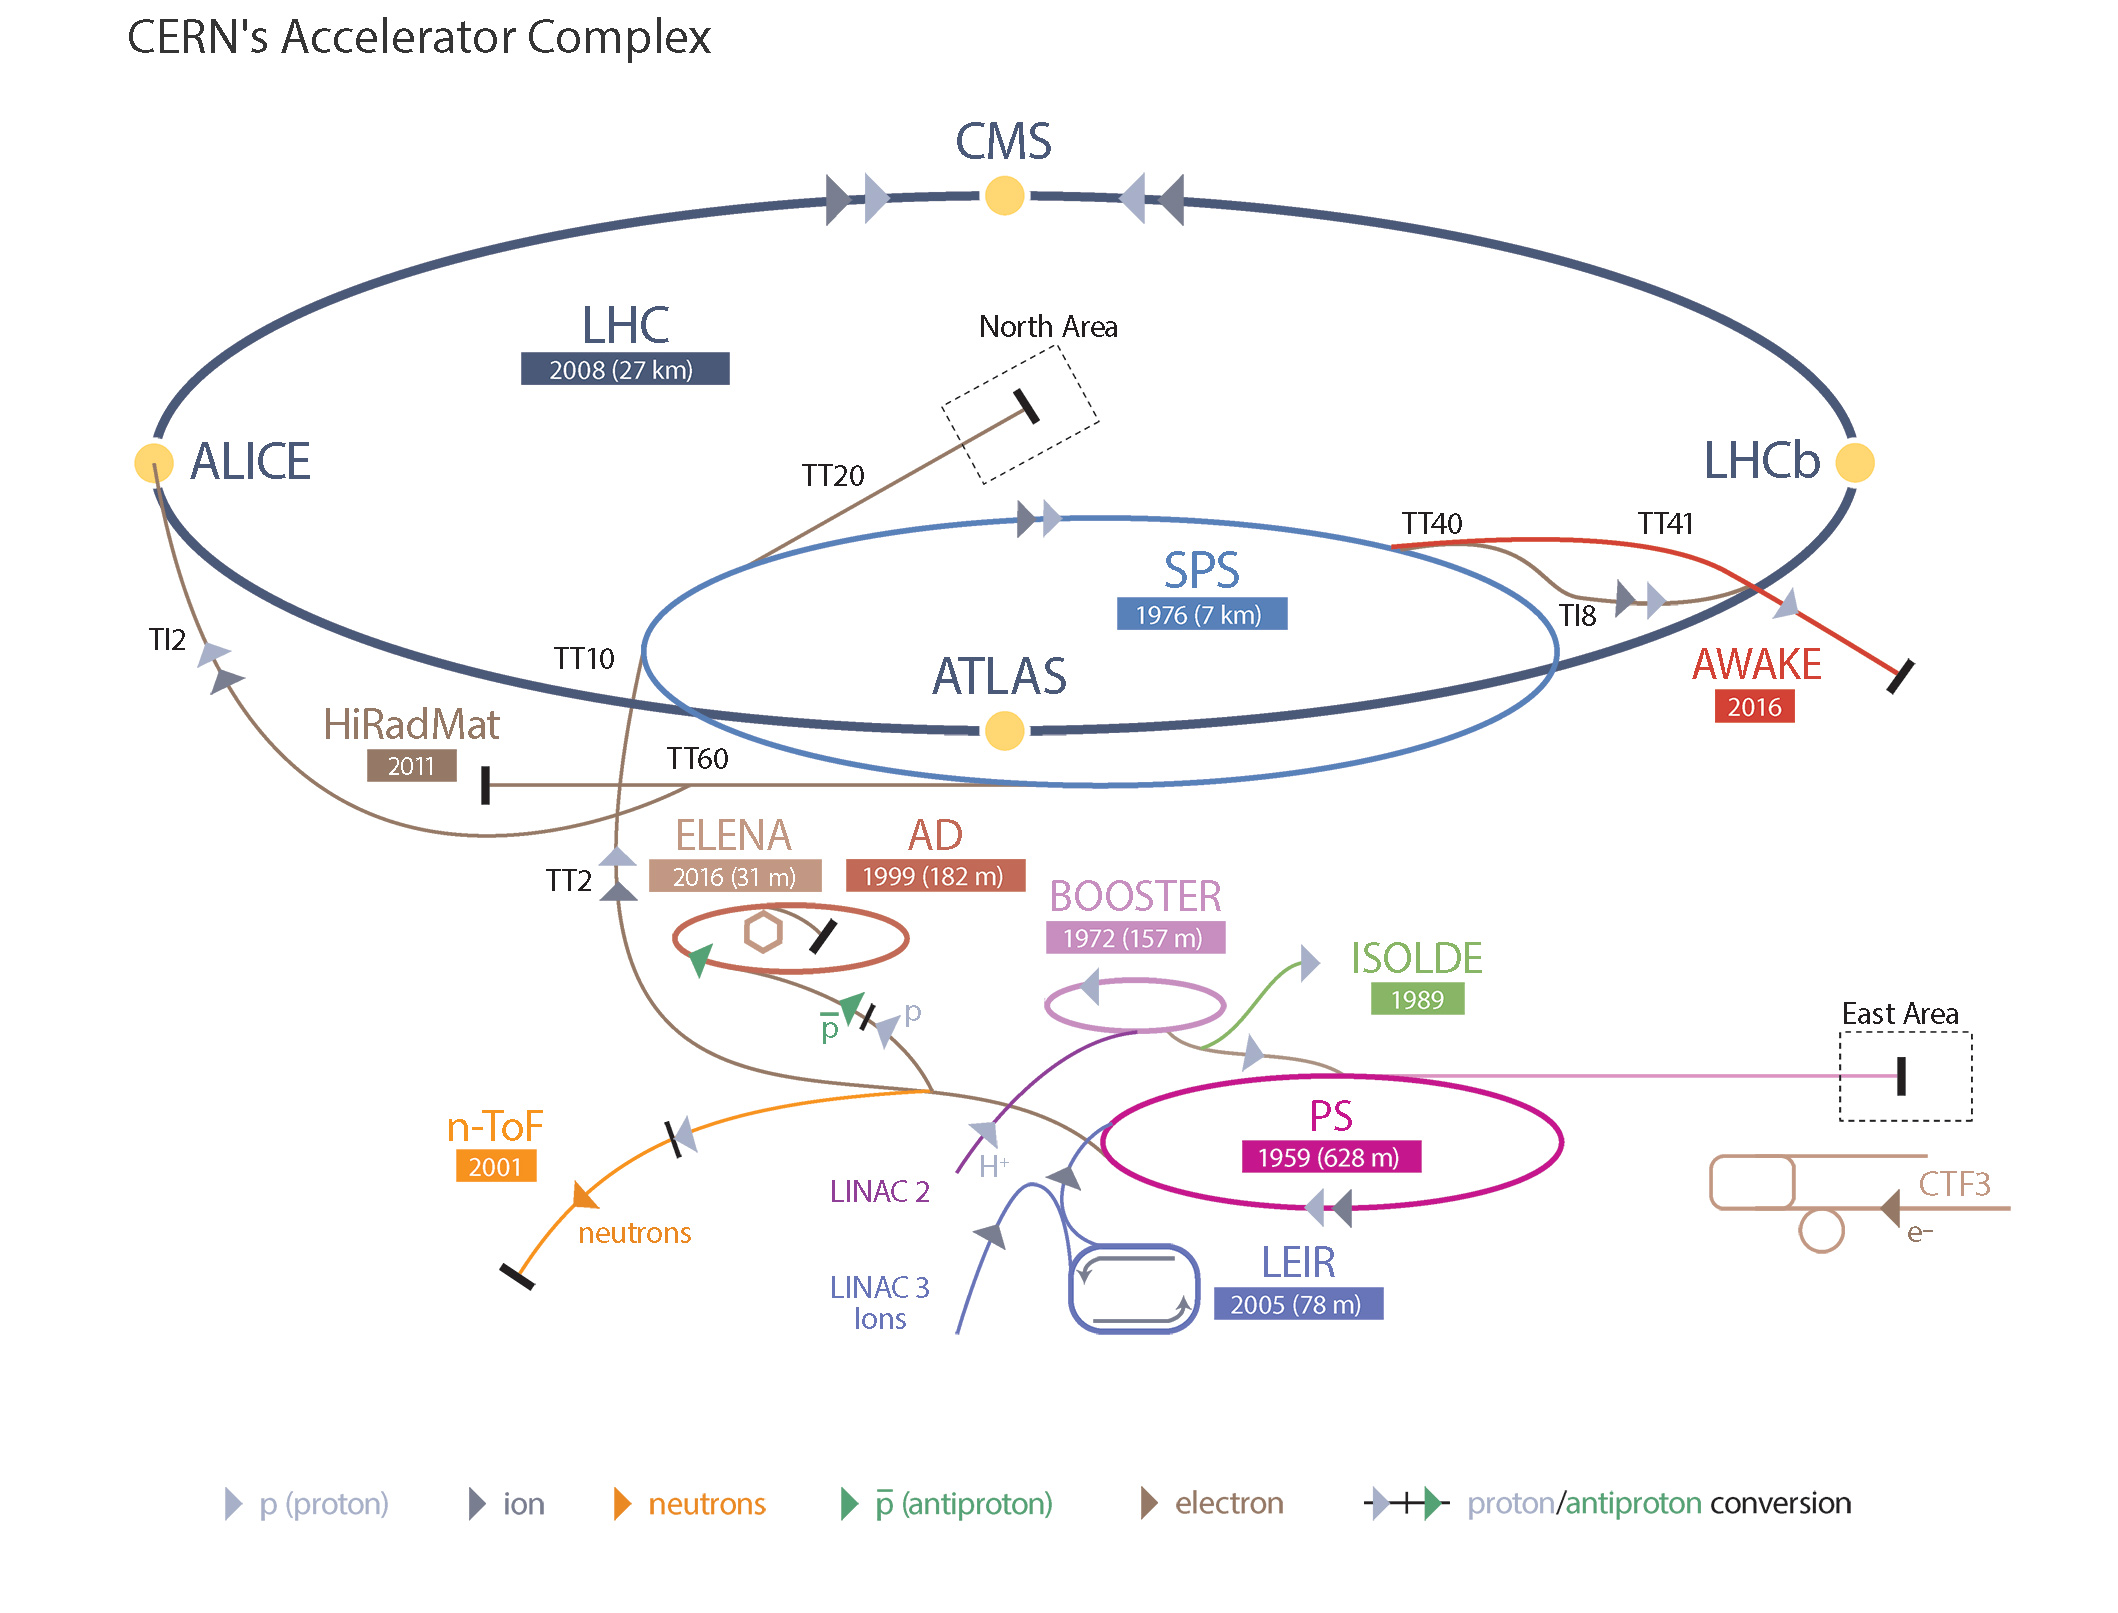
\includegraphics[width=17cm]{assets/chap02/lhc.jpg}
    \caption{The accelerator complex at CERN in Switzerland and France. Source: \cite{Marcastel:1621583}}
    \label{fig:lhc}
\end{figure}

The LHC operation consists so far of two runs: in Run 1 beginning in 2010, the first collisions at a center-of-mass energy of $\sqrt{s}=\SI{3.5}{TeV}$ started. The center-of-mass energy was upgraded in 2012 to $\sqrt{s}=\SI{8}{TeV}$. After a shutdown from 2013 to 2015, Run 2 began in 2015 at $\sqrt{s}=\SI{13}{TeV}$. The LHC will shut down by the end of 2018 to enter Run 3 at $\sqrt{s}=\SI{14}{TeV}$ in 2021.

Each of the four interaction point hosts one or multiple experiments. The most important ones are:
\begin{itemize}
\item \textbf{ATLAS} - A Toroidal LHC Apparatus
\item \textbf{CMS} - Compact Muon Solenoid
\item \textbf{ALICE} - A Large Ion Collider Experiment
\item \textbf{LHCb} - Large Hadron Collider beauty
\end{itemize}
An overview of the LHC structure is given in Figure \ref{fig:lhc}.

The performance of a particle accelerator is quantified by the luminosity, which expresses the ratio between the event rate $\dv{N}{t}$ to the interaction cross-section $\sigma$ (the probability of a process to occur)
\begin{equation}
    L=\frac{1}{\sigma} \dv{N}{t}.
\end{equation}
The larger the luminosity, the more likely an event of interest is to happen within a period of time.

\section{The Compact Muon Solenoid Experiment}
\begin{figure}[!b]
    \centering
    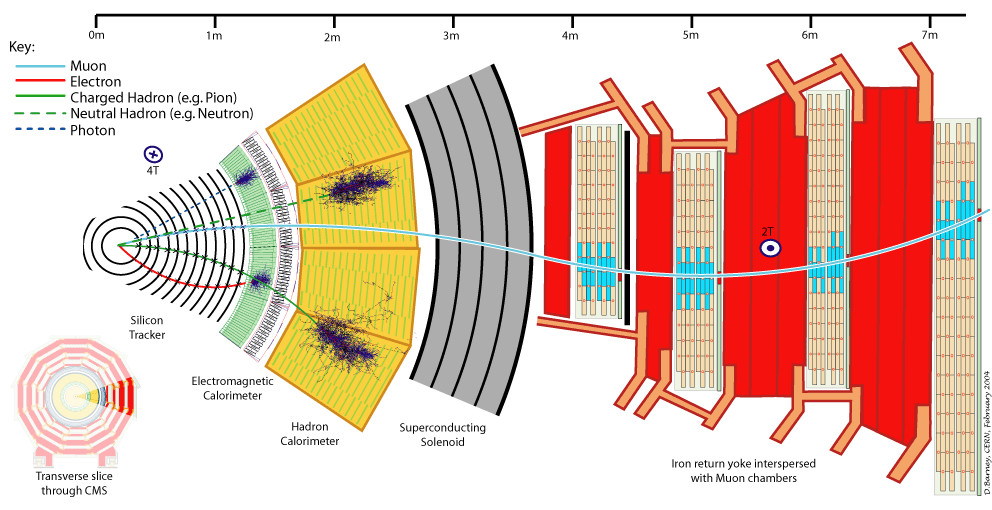
\includegraphics[width=15cm]{assets/chap02/cms.jpeg}
    \caption{Cross section view of the CMS detector and its components. Source: \cite{Davis:2205172}}
    \label{fig:cms}
\end{figure}
The Compact Muon Solenoid (CMS) is a general-purpose particle detector built into the LHC, situated in an underground cavern at Cessy, France. Its design goal was to investigate a wide range of physics, such as TeV-scale physics, the properties of the Higgs boson, heavy ion collisions, physics beyond the SM (supersymmetry, extra dimensions). It has a length of \SI{28.7}{m}, a diameter of \SI{15}{m} and a weight of approximately \SI{14000}{t}. Figure \ref{fig:cms} shows a cross section view of the CMS detector.

The detector takes its name after its relatively small size, its muon tracking ability and powerful solenoid magnet.

The CMS detector is cylindrically symmetric towards the beam axis with the interaction point centrally located. The coordinate system is oriented such that the $z$ axis is in the direction of the beam, the polar angle $\theta$ is defined in the $r$-$z$ plane with the pseudorapidity defined as $\eta=-\ln{\tan{(\theta / 2)}}$. The momentum component transverse to the beam direction, $p_{\text{T}}$, is derived from the $x$- and $y$-components, the transverse energy is defined as $E_{\text{T}}=E \sin{\theta}$ \cite{Spannagel2017}.

The inside of the detector is permeated by a \SI{3.8}{T} magnetic field parallel to the beam axis, created by the solenoid magnet, which deflects all charged particles within the detector in a helical path.

The components of the CMS from the point of interaction to its extremities are as follows \cite{Bayatian:922757}:
\begin{itemize}
    \item \textbf{The Silicon Tracker} is made of silicon pixels and microstrip detectors, which measure the paths of particles traveling outwards from the interaction point. As they pass through the tracker, charged particles create electron-hole pairs in the semiconducting material, which lead to tiny electric signals that are amplified and detected. The charge and momentum of the particle can be inferred from the curvature of the reconstructed path. The tracker is limited to detecting only particles with $|\eta|<2.5$. In order to avoid distortions in momentum measurements, the tracker was designed to reduce the interactions of particles with the tracker material.
    \item \textbf{The Electromagnetic Calorimeter} measures the energy of photons, electrons, and positrons by fully absorbing their energy. Lead tungstate crystals are used as absorber material, whose atoms can be excited by the absorption of secondary particles. The crystal leaves the excited state when photons are emitted. The intensity of the scintillation light is proportional to the energy of the absorbed particle and can be measured using photodetectors.
    \item \textbf{The Hadron Calorimeter} measures the energy of hadrons, i.e. protons, neutrons, pions, and kaons. It is made of alternating layers of absorber material and plastic scintillators. The incoming particles create a cascade of secondary particles within the absorber that cause the scintillators to emit light.
    \item \textbf{The muon system} reconstructs the paths of muons, similar to the silicon tracker. The muon detectors are located outside the solenoid. Due to their large mass compared to electrons, muons pass the inner components of the detector with negligible energy loss.
\end{itemize}

The CMS detector cannot detect neutrinos, since they barely interact with matter. This is done indirectly exploiting momentum conservation, where the sum of the transverse momenta of the collision products must vanish. The transverse momentum of the neutrinos thus equals the negative sum of the transverse momenta of the detected collision products. Assuming the neutrinos are massless, their transverse momenta equal their energy. This is also known as missing transverse energy (MET)
\begin{equation}
\slashed{E}_T=|-\sum{\va{p_\text{T}}}|.
\end{equation}

The LHC has a nominal bunch crossing frequency of about \SI{40}{MHz} with approximately 1 megabyte of data for every crossing at each interaction point. This leads to a data rate of 40 terabytes per second, which is very large given the available bandwidth out of the detector and disk space, moreover the data contains mostly physically uninteresting events. The trigger system of CMS detector reduces the event rate from \SI{40}{MHz} to \SI{1}{kHz} in two stages, making their transfer and storage feasible.

The first stage are the Level-1 (L1) triggers, which are realized by hardware electronics and filter out information from the calorimeters and the muon chambers, with only a few features of interest such as high energy jets, muons or missing energy being calculated. The triggers select events with hard scattering, and reduce the frequency by a factor of 400 to \SI{100}{kHz}. Afterwards, an online reconstruction with performance optimizations is run. This stage takes around \SI{1}{\micro s} to complete.

The second stage are the High Level Triggers (HLTs), which reduce the event rate by a further factor of 100 to \SI{1}{kHz}. The event data is then stored on tape for more detailed analysis. This trigger is software-based (mainly C++) and does complex calculations and a more precise reconstruction.
\chapter{Artificial Neural Networks}
\label{ch:nn_mva}
This chapter provides a practical introduction to artificial neural networks as the multivariate technique that was used in this work.

Artificial neural networks (ANN) represent a class of algorithms widely used in machine learning and pattern recognition, modeled after the structure of the biological brain. The power of ANNs lies in being able to identify complex relationships between given inputs and outputs, recognizing them in other input values and generating an accurate prediction.

ANNs consist of a sequence of layers containing neurons. The first layer is the \emph{input layer} with $n$ neurons, accepting input values $\va{x}=(x_1,x_2,...,x_n)$. These neurons forward the input values to the neurons of the next layer. The last layer is the \emph{output layer}, which returns the predicted values of the ANN. Between these layers, one or more \emph{hidden layers} may exist.

The type of neural networks used in the thesis is a feed-forward neural network, illustrated in Figure \ref{fig:neural_network}, where the output values are passed on from one layer to the next and do not return to any neuron of the previous layer.

\begin{figure}[h]
    \centering
    \begin{tikzpicture}[shorten >=1pt,->,draw=black!50, node distance=\layersep]
    \tikzstyle{every pin edge}=[<-,shorten <=1pt]
    \tikzstyle{neuron}=[circle,fill=black!25,minimum size=17pt,inner sep=0pt]
    \tikzstyle{input neuron}=[neuron, fill=green!50];
    \tikzstyle{output neuron}=[neuron, fill=red!50];
    \tikzstyle{hidden neuron}=[neuron, fill=blue!50];
    \tikzstyle{annot} = [text width=4em, text centered]

    % Draw the input layer nodes
    \foreach \name / \y in {1,...,4}
    % This is the same as writing \foreach \name / \y in {1/1,2/2,3/3,4/4}
        \node[input neuron] (I-\name) at (0,-\y) {};

    % Draw the hidden layer nodes
    \foreach \name / \y in {1,...,5}
        \path[yshift=0.5cm]
            node[hidden neuron] (H1-\name) at (\layersep,-\y cm) {};

    % Draw the hidden layer nodes
    \foreach \name / \y in {1,...,5}
        \path[yshift=0.5cm]
            node[hidden neuron] (H2-\name) at (2*\layersep,-\y cm) {};

    % Draw the output layer node
    \node[output neuron,pin={[pin edge={->}]right:Output}, right of=H2-3] (O) {};

    % Connect every node in the input layer with every node in the
    % hidden layer.
    \foreach \source in {1,...,4}
        \foreach \dest in {1,...,5}
            \path (I-\source) edge (H1-\dest);

    % Connect every node in the input layer with every node in the
    % hidden layer.
    \foreach \source in {1,...,5}
        \foreach \dest in {1,...,5}
            \path (H1-\source) edge (H2-\dest);

    % Connect every node in the hidden layer with the output layer
    \foreach \source in {1,...,5}
        \path (H2-\source) edge (O);

    % Annotate the layers
    \node[annot,above of=H1-1, node distance=1cm] (hl1) {Hidden layer 1};
    \node[annot,above of=H2-1, node distance=1cm] (hl2) {Hidden layer 2};
    \node[annot,left of=hl1] {Input layer};
    \node[annot,right of=hl2] {Output layer};
\end{tikzpicture}
    \caption{Example of a fully-connected neural network with one input layer containing 4 input neurons, two hidden layers containing 5 neurons each and one output layer containing a single neuron. The output of a neuron serves as input for all the neurons of the next layer.}
    \label{fig:neural_network}
\end{figure}

A feed-forward neural network with one input layer, at least one hidden layer, and one output layer is generally known as a multi-layer perceptron. A single-layer perceptron has only a single layer of output nodes, the inputs are directly fed to the outputs via a series of weights. ANNs with two hidden layers or more are known as deep neural networks (DNN).

A neuron is a single computational unit that receives the input values $\va{x}=(x_1,x_2,...,x_n)$ from all neurons in the previous layer and outputs a single value $y$ by the rule
\begin{equation}
    y=f\left( \sum_{k=1}^{n} w_k \cdot x_k + b_k \right).
\end{equation}
Each input value $x_k$ is multiplied with adaptable weights $w_k$ and an adaptable bias $b_k$ is added. An activation function $f$ is applied to the result, which introduces non-linear properties to the neuron. Without the activation function, the neural network would simply be a linear regression model and would not be able to learn and model complex data sets \cite{activationfunctions}. Commonly used activation functions are the ReLu (rectified linear unit), Elu (exponential linear unit) and sigmoid function.

\section{Training}
To calculate the correct neuron weights and biases, an ANN needs to be trained with a set of predefined input and output values (supervised learning). The available training data is split into \emph{training}, \emph{validation} and \emph{test} data. The training and validation data are both used during training, with validation data being used for determining overfitting, e.g., an accuracy increase over the training data, but an unchanged accuracy over validation data being such an indication. The testing data set is applied to the neural network after training to confirm its predictive power \cite{2976452}.

A loss or cost function $C$ that measures the inconsistency between predicted value $\hat{y}$ and actual label $y$ is used to adapt the weight $w$, such that the value of the loss function is minimized (or reaches 0). 

Examples of loss functions are the mean squared error (MSE)
\begin{equation}\label{eq:mse}
C_{\text{MSE}}=\frac{1}{N} \sum_{i=1}^N (y_i-\hat{y}_i)^2,
\end{equation}
and the binary cross entropy
\begin{equation}\label{eq:cross_entropy}
C_{\text{E}}=-\sum_{i=1}^N \left(y_i-\ln{(\hat{y}_i)+(1-y_i)\ln{(1-\hat{y}_i)}}\right),
\end{equation}
where $N$ denotes the number of the training data sets in both equations.

The optimization of the loss function is done with algorithms, such as gradient descent, stochastic gradient descent, Adam optimizer \cite{DBLP:journals/corr/KingmaB14} and others.

The step size, by which the weights are adjusted, is called the \emph{learning rate} $\eta$, and must be fine-tuned before the training
\begin{equation}\label{eq:learnrate}
    w \rightarrow w - \eta \dv{C}{w}.
\end{equation}
Higher learning rates make it difficult to determine the minimum of the cost function accurately, whereas lower learning rates may impact the performance of the algorithm. The weight readjustment as per equation \ref{eq:learnrate} is repeated for several epochs. An epoch is a full training cycle, where every element in the training data set is learned by the ANN. If $\dv{C}{w}$ is zero, a minimum or a saddle point has been reached. To avoid saddle points or shallow local minimums, the training data sample is split into batches and the weights per equation \ref{eq:learnrate} are readjusted for every batch.

The most common algorithm for weight adjustment is the backpropagation algorithm \cite{Rumelhart:1988:LRB:65669.104451}. In very broad terms, backpropagation iteratively adjusts each weight in the network proportionally to its overall error contribution. Starting at the output layer and going backwards, the chain rule of differentiation is applied for finding the derivatives of the cost function.

\section{Regularization}
\label{sec:ch_3_regularization}
Regularization is one of the many techniques used to prevent an ANN from overfitting. It consists of several methods that force the model of the ANN to be simpler. Overfitting occurs when the ANN approximates the training data too closely by losing its generalizability and abstraction ability.

The regularization methods used in this work are explained in the following.

Early stopping \cite{Prechelt2012} interrupts the training of an ANN when a monitored value does not improve after a certain number of epochs. The monitored value in this thesis is the validation loss. The available data is divided in training and validation data set. After every epoch, the validation loss is calculated by evaluating the loss function on the validation data set, and the ANN parameters, where the validation loss becomes minimal, are stored. Additionally, early stopping was combined with the learning-rate-reduction-on-plateau strategy to reduce the learning rate hyperparameter of the ANN by a certain factor if the validation loss does not improve for several epochs.

Dropout \cite{DBLP:journals/corr/abs-1207-0580} deactivates random neurons for every batch update, preventing single neurons from carrying most or all the generalization information of the ANN. This forces the network to reapply weights to the remaining active neurons making it more capable of generalizing beyond the training set. The dropout rate is used to indicate the fraction of neurons to be deactivated.

Batch normalization \cite{DBLP:journals/corr/IoffeS15} addresses the issue of \emph{internal covariance shift} by normalizing each neuron's output $y_i$. Internal covariance shift happens due to the distribution change in each layer's inputs during training, as the parameters of the previous layers change. The normalization is given by
\begin{equation}
    \hat{y}_i=\gamma \frac{y_i - \mu_\text{B}}{\sqrt{\sigma_\text{B}^2 + \epsilon}}+\beta,
\end{equation}
where $\gamma$ is an adjustable scale factor, $\beta$ an adjustable shift factor, $\sigma_\text{B}$ the standard deviation and $\mu_B$ the mean of the current training batch. Batch normalization eliminates the need for dropout in some cases, allows for much higher learning rates and speeds up training, since the input values are more within the domain of the common activation functions.

\section{Classifier Evaluation}
\label{sec:ch_3_eval}
Two of the many methods available for evaluating a classifier used in this work are the Receiver Operating Characteristics (ROC) curve and the confusion (error) matrix.

ROC graphs are two-dimensional graphs in which the true positive rate (TPR) is plotted on the $y$ axis and the false positive rate (FPR) is plotted on the $x$ axis. The ROC curve shows the trade-off between the TPR and the FPR. The integral of the curve, also known as the area-under-curve (AUC), is a measure of the accuracy of the model. The closer the curve to the diagonal, the less accurate a model is. A model with perfect accuracy will have an AUC score of 1.0, a model making random guesses, on the other hand, an AUC score of 0.5. Figure \ref{fig:ch_3_roc} shows an example ROC curve.
\begin{figure}[H]
    \centering
    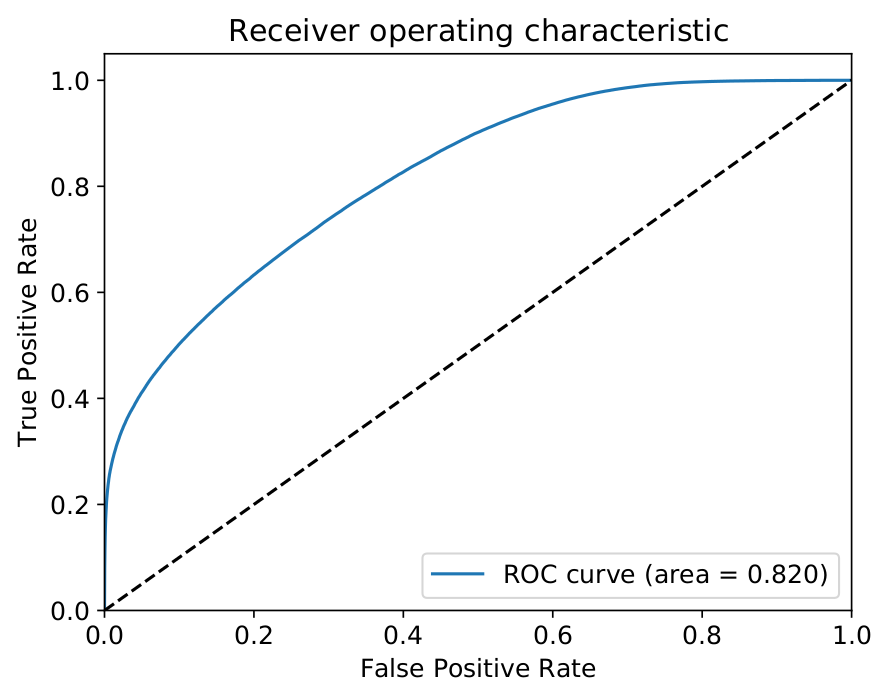
\includegraphics[width=8cm]{assets/chap03/roc.png}
    \caption{Example of a ROC curve.}
    \label{fig:ch_3_roc}
\end{figure}
The AUC score of a ROC curve can be used to determine overfitting, e.g., when the AUC score of the training data set is higher than that of the validation data set.

The confusion matrix is a table layout, where each row of the matrix represents the instance counts in a predicted class, while each column represents the counts in an actual class.

Assume a classifier has been trained to distinguish between cats, dogs and rabbits with a sample of 27 animals, where 8 are cats, 6 dogs and 13 rabbits.

\begin{table}[h]
    \caption[Confusion matrix]{Confusion matrix with prediction results of the classifier that distinguishes between cats, dogs and rabbits. Source: \cite{wiki:confusionmatrix}}
    \label{tab:ch_3_confusion_matrix}
    \begin{center}
        \begin{tabular}{|c|c|c|c|c|}
            \hhline{~~---}
            \multicolumn{2}{c|}{}&\multicolumn{3}{c|}{\textbf{Actual class}}\\
            \hhline{~~---}
            \multicolumn{2}{c|}{}&\textbf{Cat}&\textbf{Dog}&\textbf{Rabbit}\\
            \hline
            \multirow{3}{*}{\rotatebox[origin=c]{90}{\textbf{\shortstack{Predicted\\class}}}} & \textbf{Cat} & \textbf{5} & 2 & 0\\
            \hhline{~----}
             & \textbf{Dog} &3&\textbf{3}&2\\
            \hhline{~----}
             & \textbf{Rabbit} &0&1&\textbf{11}\\
            \hline
        \end{tabular}
    \end{center}
\end{table}

Reading the columns of Table \ref{tab:ch_3_confusion_matrix} vertically, the classifier predicted that of the 8 actual cats 3 were dogs, of the actual 6 dogs 2 were cats and 1 rabbit and of the actual 13 rabbits 2 were dogs. The correct predictions are highlighted in bold in the diagonal of the table, the incorrect predictions are represented by values outside the diagonal.
\chapter{Conclusion and Outlook}
Identifying single top quarks produced in the $s$-channel helps probe the electroweak sector of the standard model for deviations that may hint to physics beyond the standard model. Since the cross-section for single top quark production in the $s$-channel is almost negligible compared to those of other production modes, a promising approach in reconstructing them is using multivariate tools to build models from standard model theory predictions and apply them to real measurements from the CMS experiment.

This thesis dealt with building a deep neural network classifier, that improves the reconstruction of the single top quark in the $s$-channel at the CMS at a center-of-mass energy of \SI{13}{TeV} in the 2j2t signal region compared to the best-mass method by over \SI{7}{\%}. Simulation events for the year 2017 are used to train and evaluate the classifier.

This result is merely a first attempt and may be significantly improved upon in future work. First, some of the variables ranked by importance in Appendix \ref{ch:appendix_c} should be tried as classifier input variables by building upon the inputs that provided the highest improvement. Secondly, more meaningful variables may be used or derived. Thirdly, more hyperparameter optimization techniques should be tried out, i.e. random-search, genetic algorithms, breeding or Bayesian optimization. The tested grid search approach proves to be inefficient, as few hyperparameter values out of the many possibilities can be explored. A number of promising frameworks that take labeled data and generate the entire network topology with little or no supervision has been emerging and should be tried out.

In future work, the developed classifier should be tested with CMS experiment measured data, as well as on how effectively it can separate signal from background events for both simulation and data.


%% --------------------
%% |   Bibliography   |
%% --------------------
\cleardoublepage
\phantomsection
\addcontentsline{toc}{chapter}{\bibname}

\begingroup
\setlength{\emergencystretch}{.5em}
\printbibliography
\endgroup

%% ----------------
%% |   Appendix   |
%% ----------------
\cleardoublepage

\chapter{Input variables with the best reconstruction improvement}
\label{ch:appendix_a}
The following tables list all input variables, for which a top quark reconstruction improvement of more than \SI{4}{\%} was achieved by using the DNN classifier compared to the best-mass method introduced in Section \ref{sec:ch-4-best-mass}.

\begin{table}[h]
    \centering
    \label{tab:app_vars_1}
    \caption{Classifier input variables with which the highest reconstruction improvement was achieved.}
    \begin{tabular}{ |c|@{}c@{}| }
        \hline
        \textbf{Improvement} & \textbf{Variables}\\
        \hline
        \SI{7.83}{\%} & 
        \begin{tabular}{ll}
            \hline
            Variable & Description\\
            \hline
            $p_\text{T}\text{(j}_\text{1}$) & Transverse momentum of jet 1\\
            $\eta\text{(j}_\text{1}$) & Pseudorapidity of jet 1\\
            $\phi\text{(j}_\text{1}$) & Azimuthal angle of jet 1\\
            $m_0\text{(j}_\text{1}$) & Invariant mass of jet 1\\

            $p_\text{T}\text{(j}_\text{2}$) & Transverse momentum of jet 2\\
            $\eta\text{(j}_\text{2}$) & Pseudorapidity of jet 2\\
            $\phi\text{(j}_\text{2}$) & Azimuthal angle of jet 2\\
            $m_0\text{(j}_\text{2}$) & Invariant mass of jet 2\\

            $\Delta R \text{(j}_\text{1}\text{, W)}$ & Distance between jet 1 and the \PW boson\\
            $\Delta R \text{(j}_\text{1}\text{, lep)}$ & Distance between jet 1 and the lepton\\
            $\Delta R \text{(j}_\text{2}\text{, W)}$ & Distance between jet 2 and the \PW boson\\
            $\Delta R \text{(j}_\text{2}\text{, lep)}$ & Distance between jet 2 and the lepton\\
            \hline
        \end{tabular}\\
        \hline
    \end{tabular}
\end{table}

\begin{table}[h]
    \centering
    \label{tab:app_vars_2}
    \caption{Classifier variables that delivered the second best improvement. The \PW boson coordinates were added, the distances between the jets and the leptons were removed.}
    \begin{tabular}{ |c|@{}c@{}| }
        \hline
        \textbf{Improvement} & \textbf{Variables}\\
        \hline
        \SI{5.02}{\%} & 
        \begin{tabular}{ll}
            \hline
            Variable & Description\\
            \hline
            $p_\text{T}\text{(j}_\text{1}$) & Transverse momentum of jet 1\\
            $\eta\text{(j}_\text{1}$) & Pseudorapidity of jet 1\\
            $\phi\text{(j}_\text{1}$) & Azimuthal angle of jet 1\\
            $m_0\text{(j}_\text{1}$) & Invariant mass of jet 1\\

            $p_\text{T}\text{(j}_\text{2}$) & Transverse momentum of jet 2\\
            $\eta\text{(j}_\text{2}$) & Pseudorapidity of jet 2\\
            $\phi\text{(j}_\text{2}$) & Azimuthal angle of jet 2\\
            $m_0\text{(j}_\text{2}$) & Invariant mass of jet 2\\

            $\Delta R \text{(j}_\text{1}\text{, W)}$ & Distance between jet 1 and the \PW boson\\
            $\Delta R \text{(j}_\text{2}\text{, W)}$ & Distance between jet 2 and the \PW boson\\

            $p_\text{T}\text{(W)}$ & Transverse momentum of the \PW boson\\
            $\eta\text{(W)}$ & Pseudorapidity of the \PW boson\\
            $\phi\text{(W)}$ & Azimuthal angle of the \PW boson\\
            $m_0\text{(W)}$ & Invariant mass of the \PW boson\\
            \hline
        \end{tabular}\\
        \hline
    \end{tabular}
\end{table}

\begin{table}[h]
    \centering
    \label{tab:app_vars_3}
    \caption{Variables with the third best improvement. The distances between the jets and the lepton were added.}
    \begin{tabular}{ |c|@{}c@{}| }
        \hline
        \textbf{Improvement} & \textbf{Variables}\\
        \hline
        \SI{4.77}{\%} & 
        \begin{tabular}{ll}
            \hline
            Variable & Description\\
            \hline
            $p_\text{T}\text{(j}_\text{1}$) & Transverse momentum of jet 1\\
            $\eta\text{(j}_\text{1}$) & Pseudorapidity of jet 1\\
            $\phi\text{(j}_\text{1}$) & Azimuthal angle of jet 1\\
            $m_0\text{(j}_\text{1}$) & Invariant mass of jet 1\\

            $p_\text{T}\text{(j}_\text{2}$) & Transverse momentum of jet 2\\
            $\eta\text{(j}_\text{2}$) & Pseudorapidity of jet 2\\
            $\phi\text{(j}_\text{2}$) & Azimuthal angle of jet 2\\
            $m_0\text{(j}_\text{2}$) & Invariant mass of jet 2\\

            $\Delta R\text{(j}_\text{1}\text{, W)}$ & Distance between jet 1 and the \PW boson\\
            $\Delta R\text{(j}_\text{1}\text{, lep)}$ & Distance between jet 1 and the lepton\\
            $\Delta R\text{(j}_\text{2}\text{, W)}$ & Distance between jet 2 and the \PW boson\\
            $\Delta R\text{(j}_\text{2}\text{, lep)}$ & Distance between jet 2 and the lepton\\

            $p_\text{T}\text{(W)}$ & Transverse momentum of the \PW boson\\
            $\eta\text{(W)}$ & Pseudorapidity of the \PW boson\\
            $\phi\text{(W)}$ & Azimuthal angle of the \PW boson\\
            $m_0\text{(W)}$ & Invariant mass of the \PW boson\\
            \hline
        \end{tabular}\\
        \hline
    \end{tabular}
\end{table}

\begin{table}[h]
    \centering
    \label{tab:app_vars_4}
    \caption{Variables with the fourth best improvement. The transverse mass of the \PW boson was added, the distances between the jets and the lepton were removed.}
    \begin{tabular}{ |c|@{}c@{}| }
        \hline
        \textbf{Improvement} & \textbf{Variables}\\
        \hline
        \SI{4.52}{\%} & 
        \begin{tabular}{ll}
            \hline
            Variable & Description\\
            \hline
            $p_\text{T}\text{(j}_\text{1}$) & Transverse momentum of jet 1\\
            $\eta\text{(j}_\text{1}$) & Pseudorapidity of jet 1\\
            $\phi\text{(j}_\text{1}$) & Azimuthal angle of jet 1\\
            $m_0\text{(j}_\text{1}$) & Invariant mass of jet 1\\

            $p_\text{T}\text{(j}_\text{2}$) & Transverse momentum of jet 2\\
            $\eta\text{(j}_\text{2}$) & Pseudorapidity of jet 2\\
            $\phi\text{(j}_\text{2}$) & Azimuthal angle of jet 2\\
            $m_0\text{(j}_\text{2}$) & Invariant mass of jet 2\\

            $\Delta R\text{(j}_\text{1}\text{, W)}$ & Distance between jet 1 and the \PW boson\\
            $\Delta R\text{(j}_\text{2}\text{, W)}$ & Distance between jet 2 and the \PW boson\\

            $p_\text{T}\text{(W)}$ & Transverse momentum of the \PW boson\\
            $\eta\text{(W)}$ & Pseudorapidity of the \PW boson\\
            $\phi\text{(W)}$ & Azimuthal angle of the \PW boson\\
            $m_0\text{(W)}$ & Invariant mass of the \PW boson\\
            $m_\text{T}\text{(W)}$ & Transverse mass of the \PW boson\\
            \hline
        \end{tabular}\\
        \hline
    \end{tabular}
\end{table}

\begin{table}[h]
    \centering
    \label{tab:app_vars_5}
    \caption{Variables with the fifth best improvement --- here the transverse missing energy of the \PW boson was added.}
    \begin{tabular}{ |c|@{}c@{}| }
        \hline
        \textbf{Improvement} & \textbf{Variables}\\
        \hline
        \SI{4.45}{\%} & 
        \begin{tabular}{ll}
            \hline
            Variable & Description\\
            \hline
            $p_\text{T}\text{(j}_\text{1}$) & Transverse momentum of jet 1\\
            $\eta\text{(j}_\text{1}$) & Pseudorapidity of jet 1\\
            $\phi\text{(j}_\text{1}$) & Azimuthal angle of jet 1\\
            $m_0\text{(j}_\text{1}$) & Invariant mass of jet 1\\

            $p_\text{T}\text{(j}_\text{2}$) & Transverse momentum of jet 2\\
            $\eta\text{(j}_\text{2}$) & Pseudorapidity of jet 2\\
            $\phi\text{(j}_\text{2}$) & Azimuthal angle of jet 2\\
            $m_0\text{(j}_\text{2}$) & Invariant mass of jet 2\\

            $\Delta R\text{(j}_\text{1}\text{, W)}$ & Distance between jet 1 and the \PW boson\\
            $\Delta R\text{(j}_\text{2}\text{, W)}$ & Distance between jet 2 and the \PW boson\\

            $p_\text{T}\text{(W)}$ & Transverse momentum of the \PW boson\\
            $\eta\text{(W)}$ & Pseudorapidity of the \PW boson\\
            $\phi\text{(W)}$ & Azimuthal angle of the \PW boson\\
            $m_0\text{(W)}$ & Invariant mass of the \PW boson\\
            $m_\text{T}\text{(W)}$ & Transverse mass of the \PW boson\\
            $\text{met}_\text{T}\text{(W)}$ & Transverse missing energy of the \PW boson\\
            \hline
        \end{tabular}\\
        \hline
    \end{tabular}
\end{table}

\begin{table}[h]
    \centering
    \label{tab:app_vars_6}
    \caption{Variables with the sixth best improvement, the azimuthal angle difference between the jets and the \PW boson, the invariant mass of the jets and the \PW boson respectively were added, the transverse missing energy of the \PW boson was removed.}
    \begin{tabular}{ |c|@{}c@{}| }
        \hline
        \textbf{Improvement} & \textbf{Variables}\\
        \hline
        \SI{4.31}{\%} & 
        \begin{tabular}{ll}
            \hline
            Variable & Description\\
            \hline
            $p_\text{T}\text{(j}_\text{1}$) & Transverse momentum of jet 1\\
            $\eta\text{(j}_\text{1}$) & Pseudorapidity of jet 1\\
            $\phi\text{(j}_\text{1}$) & Azimuthal angle of jet 1\\
            $m_0\text{(j}_\text{1}$) & Invariant mass of jet 1\\

            $p_\text{T}\text{(j}_\text{2}$) & Transverse momentum of jet 2\\
            $\eta\text{(j}_\text{2}$) & Pseudorapidity of jet 2\\
            $\phi\text{(j}_\text{2}$) & Azimuthal angle of jet 2\\
            $m_0\text{(j}_\text{2}$) & Invariant mass of jet 2\\
            
            $p_\text{T}\text{(W)}$ & Transverse momentum of the \PW boson\\
            $\eta\text{(W)}$ & Pseudorapidity of the \PW boson\\
            $\phi\text{(W)}$ & Azimuthal angle of the \PW boson\\
            $m_0\text{(W)}$ & Invariant mass of the \PW boson\\

            $\Delta R(\text{j}_\text{1}\text{, W)}$ & Distance between jet 1 and the \PW boson\\
            $\Delta \phi\text{(j}_\text{1}\text{, W)}$ & Azimuthal angle difference between jet 1 and the \PW boson\\
            $m_0\text{(j}_\text{1}\text{, W)}$ & Invariant mass of jet 1 and the \PW boson system\\
            
            $\Delta R\text{(j}_\text{2}\text{, W)}$ & Distance between jet 2 and the \PW boson\\
            $\Delta \phi\text{(j}_\text{2}\text{, W)}$ & Azimuthal angle difference between jet 2 and the \PW boson\\
            $m_0\text{(j}_\text{2}\text{, W)}$ & Invariant mass of jet 2 and the \PW boson system\\
            \hline
        \end{tabular}\\
        \hline
    \end{tabular}
\end{table}

\chapter{Plots of reconstruction improvement over average learning rate}
\label{ch:appendix_lr}
The following plots demonstrate how the average learning rate of the training of the classifier affects the reconstruction improvement in percent of the DNN over the best-mass method. The classifier topology and its input variables differ slightly in every training instance below. In one instance batch normalization was used. The logarithmic learning rate that yields the best improvement appears to be in the $10^{-6}$ order of magnitude.

\begin{figure}[h]
    \centering
    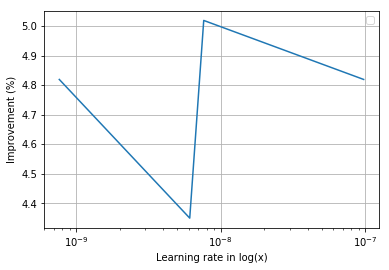
\includegraphics[width=.5\textwidth]{assets/appendix/plot_group25.png}
    \caption{Without batch normalization}
    \label{fig:ch_5_plot25}
\end{figure}
\begin{figure}[h]
    \centering
    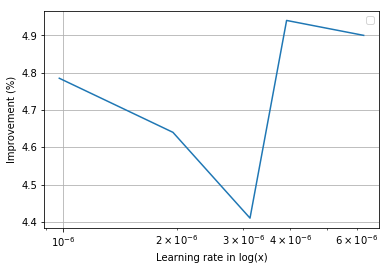
\includegraphics[width=.5\textwidth]{assets/appendix/plot_group21.png}
    \caption{With batch normalization}
    \label{fig:ch_5_plot21}
\end{figure}
\begin{figure}[h]
    \centering
    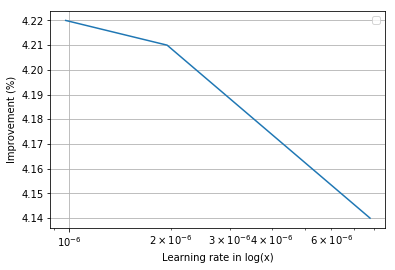
\includegraphics[width=.65\textwidth]{assets/appendix/plot_group23.png}
    \caption{Without batch normalization}
    \label{fig:ch_5_plot23}
\end{figure}
\begin{figure}[h]
    \centering
    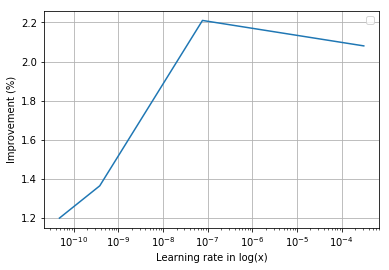
\includegraphics[width=.65\textwidth]{assets/appendix/plot_group1.png}
    \caption{Without batch normalization}
    \label{fig:ch_5_plot1}
\end{figure}
\begin{figure}[h]
    \centering
    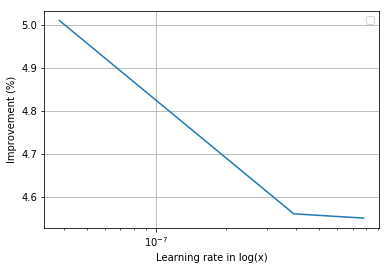
\includegraphics[width=.65\textwidth]{assets/appendix/plot_group5.png}
    \caption{Without batch normalization}
    \label{fig:ch_5_plot5}
\end{figure}

\chapter{Most significant variables according to feature selection}
\label{ch:appendix_c}
The following tables list the variables that best correlate with labeled output and may therefore possess potentially good discrimination capabilities. They were determined using the various feature selection algorithms introduced in Section \ref{sec:ch-4-input-vars}.

\npdecimalsign{.}
\nprounddigits{2}

\LTXtable{\textwidth}{assets/appendix/anova}
\LTXtable{\textwidth}{assets/appendix/rfe}
\LTXtable{\textwidth}{assets/appendix/fi}


\backmatter

\chapter*{Acknowledgments}
\chaptermark{Acknowledgments}

My thanks go to everyone from the Institute of Experimental Particle Physics at the Karlsruhe Institute of Technology, who contributed in creating a pleasant working environment, in particular to:

Prof. Dr. Thomas Müller and Dr. Thorsten Chwalek for giving me the opportunity to prepare my bachelor thesis in their working group. Particle physics research has always fascinated me --- together with space exploration they represent humanity's most elaborate efforts to date in its attempt to give answers to basic questions and find order in the universe.

Darius Bühler for taking his time to answer my many particle physics-related questions, for proofreading my thesis, and for otherwise interesting discussions.

David Walter for introducing me to the topic of machine learning and for his useful insights.

My advisor, Dr. Nils Faltermann, for his support and for proofreading my thesis.

Kevin Flöh for proofreading my thesis.

Also my family for their moral support.

\end{document}
